\documentclass[11pt]{article}


\usepackage{amsmath}
\usepackage{enumitem}
\usepackage{graphicx}
    \graphicspath{{../images/labs}}
\usepackage{ragged2e}
\usepackage[margin=0.75in]{geometry}

\begin{document}

    \begin{enumerate}
        \item A stomach cell line growing in nutrient broth has a mutation in the gene encoding a particular
type of tRNA\@. Assuming the mutation is not lethal to the cells, explain why the amount
of SIRT3 mRNA in this cell line is identical to the amount produced by a normal stomach (NS)
cell line but the amount of SIRT3 protein is less than in the NS cells.
        \begin{enumerate}
            \item There could be many reasons, however only two are likely.
            One, the stomach cell in the nutrient broth has just a point-shift or deletion mutation.
            Two, the stomach cell is cancerous, however are ineffective due to a reason unknown.
            In either case, the amount of SIRT3 produced will always be different, likely less than a functional cancerous cell.\\
            \textbf{0/1} $\rightarrow$ Looking for an explanation that tRNAs are involved in translation, not transcription.
        \end{enumerate}
        \item Identify a control group for the analysis shown in Figure~\ref{Figure 3}.
        Justify analyzing SIRT3 protein level in
        four different cancer cell lines, as shown in Figure~\ref{Figure 1}.
        Based on Figures~\ref{Figure 1} and~\ref{Figure 3}, describe the
        relationship between SIRT3 expression and cytoplasmic ATP levels.
        Calculate the percent change
        in cytoplasmic ATP levels by SC+RNA cells compared with SC+plasmid cells.
        \begin{enumerate}
            \item The control group presented in Figure~\ref{Figure 3} would be the NS, or Normal Stomach cells.
            In Figure~\ref{Figure 1}, they show 5 bars, one for the control group, NS, and 4 for the different cancer patient levels.
            The justification for having 4 different bars of levels lies in the bias of only having one average.
            Having just one average bar, let alone just one patient, would present false and misleading data.
            There seems to be a heavy correlation between having stomach cancer cells, SIRT3 protein levels, and high cytoplasmic ATP levels.
            As seen in Figure~\ref{Figure 1}, the patients with the stomach cancer cells presented higher than normal SIRT3 protein levels.
            And then in Figure~\ref{Figure 3}, the stomach cells present higher than normal cytoplasmic ATP levels.
            This indicates a fairly strong correlation between the SIRT3 protein and cytoplasmic ATP levels. \\
            \textbf{3/4} $\rightarrow$ Response included an acceptable control group, a justification for more than one cell line (small sample size).
            Explained the coorelation between SIRT3 protein levels and cytoplasmic ATP levels.
            Did not, however, explain the percent change in cytoplasmic ATP levels by SC+RNA cells compared with SC+plasmid cells.
            The answer is -59\%.
        \end{enumerate}
        \item Researchers analyzing the SIRT3 gene sequence engineer a SIRT3 gene that is identical to the
normal gene except that a single nucleotide has been deleted from the 5` end of the second
exon of the gene; the deletion does not affect splicing. The researchers introduce this gene into
normal stomach cells to determine how the primary AND tertiary structures of the protein
expressed from the engineered SIRT3 gene will compare with the protein expressed from the
normal SIRT3 gene in these cells. Predict the results of this experiment. The researchers claim
that the data in Figure 3 provide evidence that the stomach cancer cells perform fermentation
to a greater extent than do normal stomach cells. Provide reasoning to justify the claim. Based
on the information provided, predict the effect on the ratio of NADH/NAD+ in the cells treated
with the compound that blocks the electron transport chain compared with similar cells not
treated with the compound.
        \begin{enumerate}
            \item The results from the experiment are likely going to show the structures differing.
            This is due to the fact that a nucleotide was deleted, not replaced.
            And while that doesn't affect splicing, it will affect how the protein folds both its primary and tertiary structures.
            The researchers also claimed that Figure~\ref{Figure 3} provides data for cancer cells performing fermentation to a greater extent than normal cells.
            This is true, as in both the SC-1 and SC+Plasmid bars, we see an increase in lactic acid production \textemdash\ the byproduct of fermentation. \\
            \textbf{1/3} $\rightarrow$ Did not explain NADH/NAD+ relation to fermentation, or detailed other stuff. Mostly the last part of the question.
        \end{enumerate}
        \item Based on the data provided, explain how testing for SIRT3 gene expression in samples of
stomach cells might be used by physicians to predict which individuals have an increased risk of
developing stomach cancer. Human stomach cells have plasma membrane receptors for the
binding of certain extracellular signaling molecules such as growth factors. Explain why the
irreversible binding of chemicals that mimic the growth factors will most likely change the
normal cells into cancer cells.
        \begin{enumerate}
            \item Testing for SIRT3 could be used to indicate an increased risk of stomach cancer via testing for the increased levels.
            Figure~\ref{Figure 1} supports this by showing that stomach cancer cells lead to increased levels of the SIRT3 protein.
            The physicians would likely get a blood, gastric, or bile sample, looking for increased SIRT3 protein levels.
            If presented, the patient would likely be recommended for a more thorough cancer screening.
            If a chemical that mimics a growth factor or some other type of ligand were to bind to the plasma-membrane receptor, the cells would likely become cancerous.
            This is thanks to the process being irreversible.
            In other words, the ligand will~\textit{never}~detach from the receptor.
            This would in turn lead to \lq{cancerous}\rq\ activity, such as never ending production, inefficiency, and/or inflated consumption of glucose.\\
            \textbf{2/2} $\rightarrow$ Explained how a higher level of SIRT3 proteins could lead to a reccomendation for stomach cancer, and how
        \end{enumerate}
    \end{enumerate}


\newpage{

\begin{figure}
\caption{1}
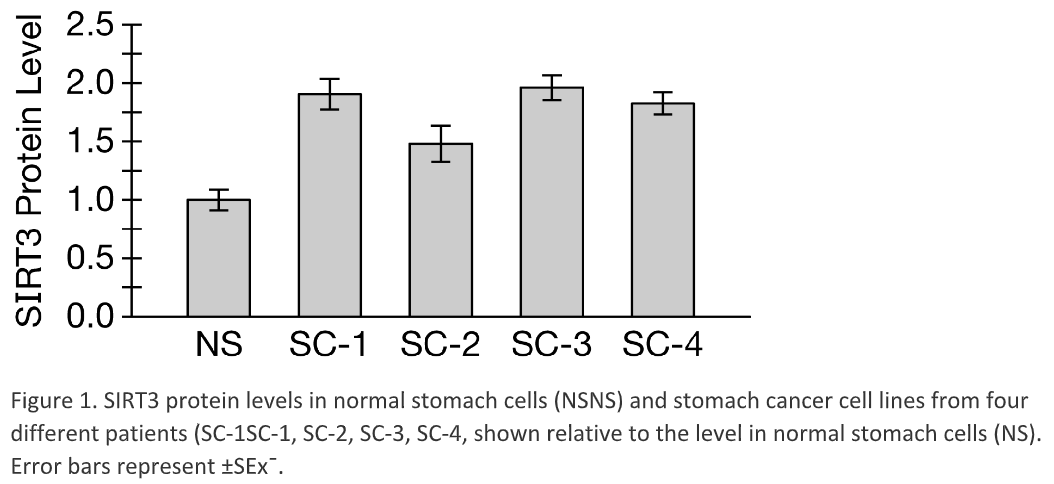
\includegraphics{Long FRQ Fig. 1}\label{Figure-1}
\end{figure}

\begin{figure}
\caption{2}
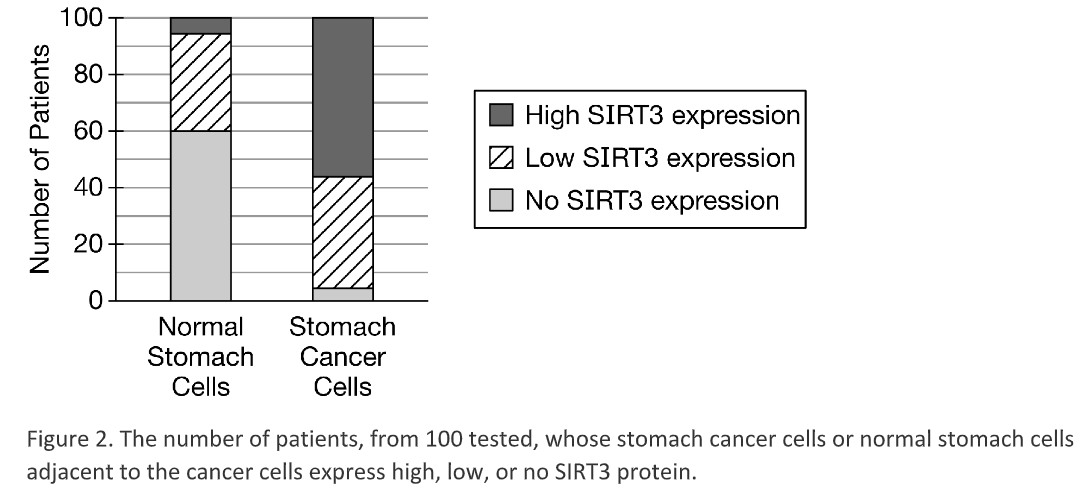
\includegraphics{Long FRQ Fig. 2}\label{Figure-2}
\end{figure}

\begin{figure}
\caption{3}
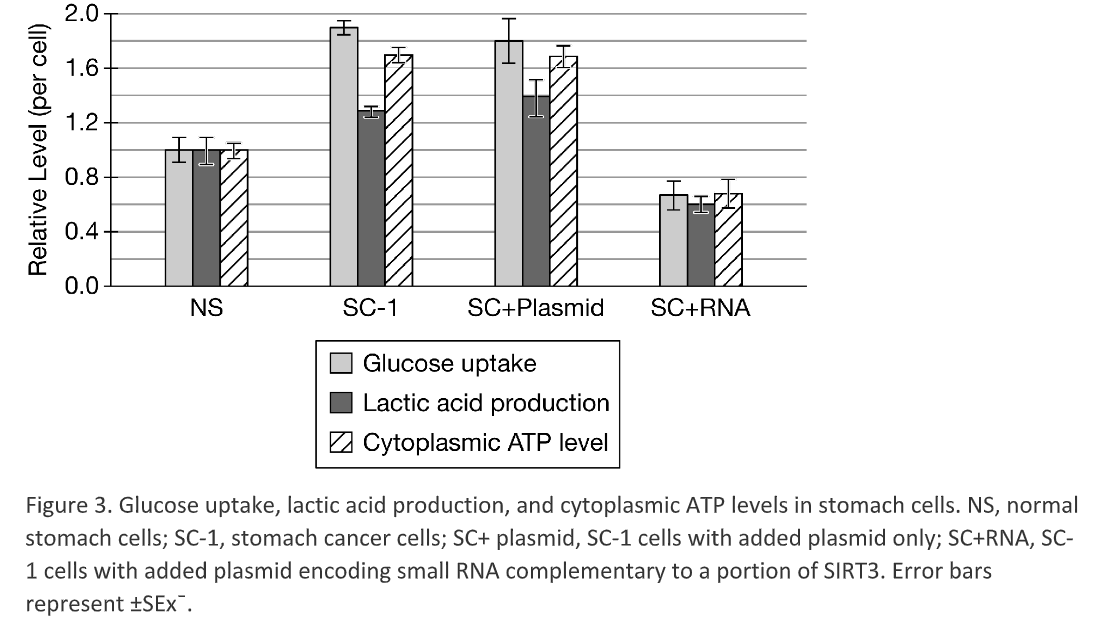
\includegraphics{Long FRQ Fig. 3}\label{Figure-3}
\end{figure}

}












\end{document}
